% % %
% Recommended compilation method:
%  $ latexmk -pdf templete_main.tex 
%
% If you use 
%  $ latexmk -pdfdvi templete_main.tex
% then you must write `dvipdfmx' in option of \documentclass, i.e.,
%  \documentclass[12pt, a4paper, openany, dvipdfmx]{book}
%
% % %

% % % Document Type
% % % Ref.: http://www.biwako.shiga-u.ac.jp/sensei/kumazawa/tex/book.html
\documentclass[11pt, a4paper, openany]{book}

% % % Necessary
\usepackage{amssymb, amsmath, latexsym}  % For mathematics [Before hyperref]
\usepackage[setpagesize=false]{hyperref} % For inserting hyperlink [Before graphicx]
\usepackage{graphicx}                    % For inserting figure
\usepackage{subcaption}                  % For caption of figures and tables
\usepackage[usenames]{color}             % For coloring
\usepackage[shortlabels]{enumitem}       % For useful enumerate and itemize environment
\usepackage{comment}                     % For commenting multiline
\usepackage{cite}                        % For citing references [After hyperref]
\usepackage{url}                         % For inserting URL
\usepackage{acro}                        % For listing abbreviations and symbols
\usepackage{master}                      % For master thesis [After graphicx and color]

% % % Convenient for tables and emphasis
\usepackage{tabularx}       % For flexible table
\usepackage{multirow}       % For combining multi rows for table
\usepackage{colortbl}       % For coloring table
\usepackage{longtable}      % For long table across multiple pages
\usepackage[normalem]{ulem} % For flexible underline etc.
\usepackage{bxascmac}       % For framing multiline
\usepackage{adjustbox}      % For adjust size of tables

% % % Option
\usepackage{siunitx}   % For using SI units
\usepackage{afterpage} % For inserting newpage
\usepackage{listings}  % For inserting programming code
\usepackage{docmute}   % For compilation of divided files
\usepackage{algorithmicx}
\usepackage{algorithm}
\usepackage{algpseudocode}
% % % Configuration for hyperlink
\hypersetup{ %
	breaklinks=true, %
	colorlinks=false, %
	urlcolor=blue, %
	urlbordercolor={0 1 1}}

% % % Define Command
\newcommand{\bm}[1]{\mbox{\boldmath $#1$}}
\newcommand{\setrow}[1]{\gdef\rowmac{#1}#1\ignorespaces}


% % % Re-define names

% % 論文題目     / Title
\title{Detecting Android malware applications using Static Analysis and Machine learning}
% % 著者名       / Author name
\author{Cristian Naoki Kamia}
% % 修了時期     / Year and month when you complete master course
\datestamp{March 2020} 
% % 主査名と職階 / Name and position of chief examiner
\mainreferee{Vitaly Klyuev}    
\mainrefereeposition{Senior Associate Professor}
% % 副査名と職階 / Name and position of deputy examiner
\secondreferee{Evgeny Pyshkin}
\secondrefereeposition{Senior Associate Professor}
\thirdreferee{Incheon Paik}
\thirdrefereeposition{Professor}

% % You can define abbreviations and symbols, if any.
% % If you show lists of either abbreviations, symbols or both, 
% % you should define them in ./Chapter/Acronym.tex
% % However, if you do not need the lists, you should comment out the following line
% % and replace \showlist command to \showlists{y}{y}{n}{n}
% % % Reference: 
% http://tex.stackexchange.com/questions/86666/how-to-create-both-list-of-abbreviations-and-list-of-nomenclature-using-nomencl
% ftp://ftp.kddilabs.jp/CTAN/macros/latex/contrib/acro/acro_en.pdf
% % %

% Configuration for hyperlink and list of acronyms
\acsetup{hyperref=true, list-style=longtable, list-heading=chapter*}

% class `abbrev': abbreviations:
\DeclareAcronym{pc}{
  short = PC ,
  long  = Personal Computer ,
  class = abbrev
}
\DeclareAcronym{apk}{
  short = APK ,
  long  = Android Package ,
  class = abbrev
}
\DeclareAcronym{uoa}{
  short = UoA,
  long  = University of Aizu,
  class = abbrev
}

\DeclareAcronym{api}{
  short = API,
  long = Application Programming Interface,
  class = abbrev
}

\DeclareAcronym{hal}{
  short = HAL,
  long = Hardware Application Layer,
  class = abbrev
}

\DeclareAcronym{art}{
  short = ART,
  long = Android Runtime,
  class = abbrev
}

\DeclareAcronym{csv}{
  short = CSV,
  long = Comma-separated values,
  class = abbrev
}

% class `nomencl': nomenclature (symbol)
\DeclareAcronym{A}{
  short = $\bm{A}$ ,
  long  = Matrix ,
  sort  = A ,
  class = nomencl
}
\DeclareAcronym{a}{
  short = $\bm{a}$ ,
  long  = Vector ,
  sort  = a ,
  class = nomencl
}
\DeclareAcronym{r}{
  short = $\mathbb{R}$ ,
  long  = Set of real numbers ,
  sort  = R ,
  class = nomencl
}



\begin{document}
% % タイトル、著作権、承認ページ、目次の作成 
% % Make pages for title, copyright, approval and table of contents
\makefrontmattar

% % 図、表、略語、記号一覧の表示
% % Show lists of figures, tables, abbreviations and symbols (Optional)
% % %
% % If you set 'n' to the fourth argument of \showlists{figures}{tables}{abbreviaions}{symbols}
% % (i.e. \showlists{y}{y}{y}{n}), list of symbols is not shown.
% % Similarly, you can decide if you show each list. 
% % %
\showlists{y}{y}{y}{n}{y}
% \showlists{y}{y}{n}{n}
% % 謝辞を挿入 / Acknowledment (Optional)
% \chapter*{Acknowledgment}
% % 要旨を挿入
\chapter*{Abstract}
% % There is no page number in abstract
\thispagestyle{empty}

Android has been intently picked as the main target by many malware creators for
designing new malicious applications. Every day, thousands of new malware samples
try to circumvent the security measures implemented by Android applications stores,
aiming to infect new devices. In order to tackle this problem, it is required to research and develop mechanisms able to classify large amounts of suspicious samples
automatically, detecting those that contain a malicious payload.

In this thesis, we proposed a novel end-to-end Android malware detection system using static features extracted from the application files to try to detect a malware application. We extracted 7 different Static features to use for input data. Also, this system uses a machine learning model implemented with several machine learning algorithms combined with our proposed Stacking method that is often used in Kaggle competitions to get the best performance of the algorithms. We evaluated our proposed system with 20,000 samples of applications downloaded from Androzoo \cite{androzoo} database. Our proposed system reach to 93.6\verb+%+ of accuracy when implementing our proposed stacking method.

% % %
% Begin of Body
% % %
\configbody

% % When you request examiners to do a peer review of your thesis, the paper should be double-spacing.
% % When you submit your thesis, the paper must be single-spacing.
%\singlespacing
\doublespacing

% % Chapterごとにファイルを分けて,それぞれをincludeする
% % You should make files of each chapter, and include them.
% % doc mute package is convenient to edit and compile each file. If you are interested, please search the package.
\chapter{Introduction}

The android operating system, which is provided by Google, is predicted to continue to have a dramatic increase in the market with around 1.5 billion Android-based devices to be shipped by 2021 sta. It is currently leading the mobile OS market with over 80\verb+%+ market share compared to iOS, Windows, Blackberry, and Symbian OS as Figure \ref{fig:marketshare}. The availability of diverse Android markets such as Google Play, the official store, and third-party markets makes Android devices a popular target to not only legitimate developers, but also malware developers. Over one billion devices have been sold and more than 65 billion downloads have been made from Google Play. Android apps can be found in different categories, such as educational apps, gaming apps, social media apps, entertainment apps, banking apps, etc.

\begin{figure}[htbp]
    \centering
    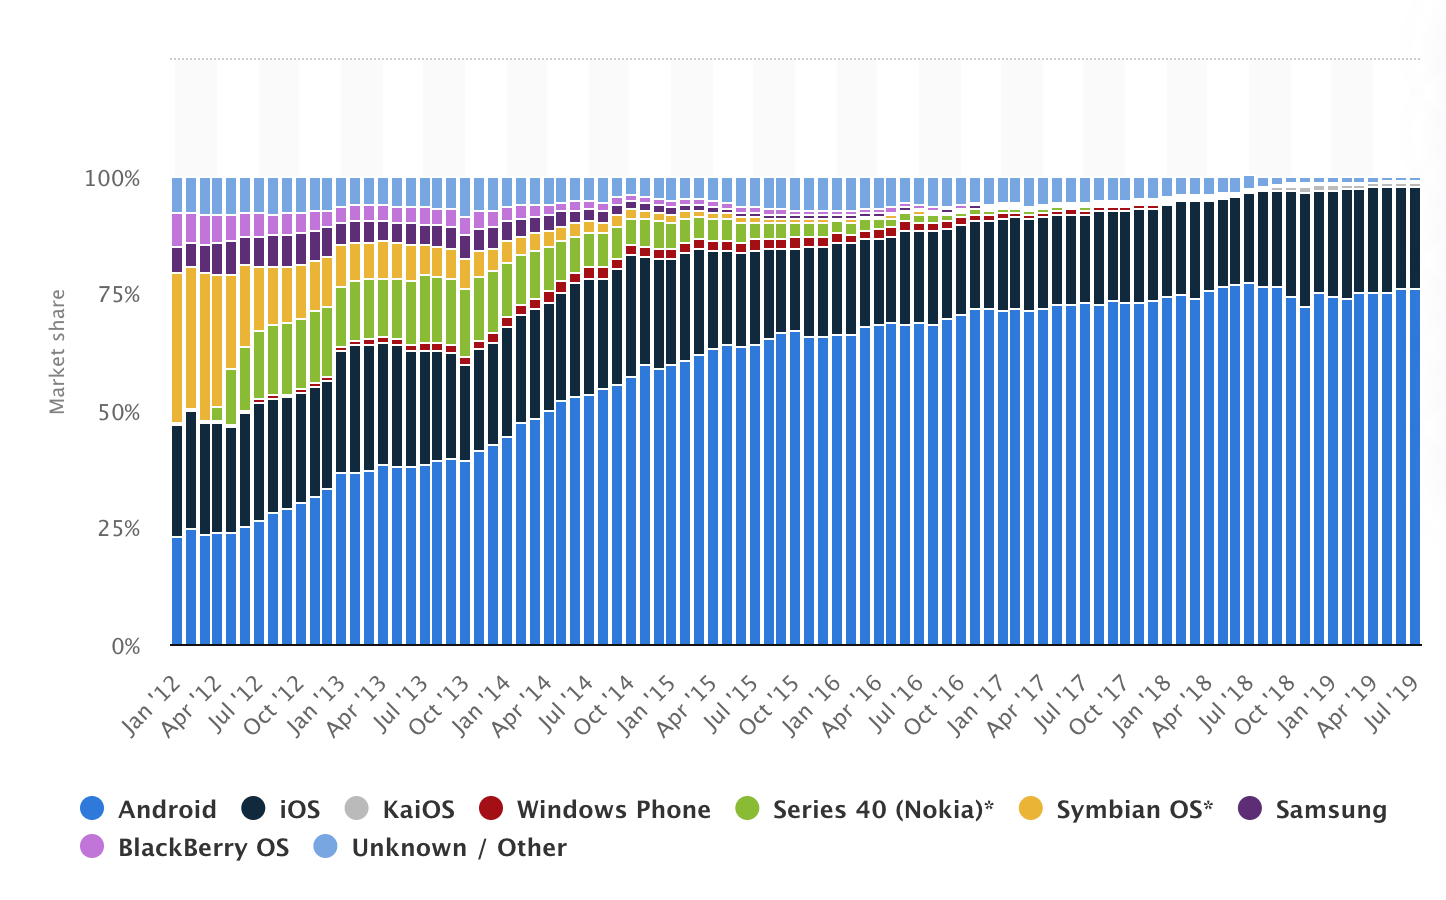
\includegraphics[scale=0.5]{./Figure/marketshare.png}
    \caption{Mobile operating systems's market share worldwide from January 2012 to July 2019 \cite{androidshare}}
    \label{fig:marketshare}
  \end{figure}

As a technology that is open source and widely adopted, Android is facing many challenges especially with malicious applications. The malware infected apps have the ability to send text messages to premium rate numbers without the user acknowledgment, gain access to private data, or even install code that can download and execute additional malware on the victim’s device. The malware can also be used to create mobile botnets \cite{dl-droid}. Over the last few years, the number of malware samples attacking Android has significantly increased as you can see at Figure \ref{fig:androidgraph}. Attacks on other connected things around the house gained momentum as well. While hidden apps and Adware remain by far the most common form of mobile threats in Android, the others are growing and learning how to infect other types of devices as well. According to a recent report from McAfee \cite{mcafee}, detections of backdoors,cryptomining, fake apps, and banking Trojans all
increased substantially in the latter half of the year. 

\begin{figure}[htbp]
    \centering
    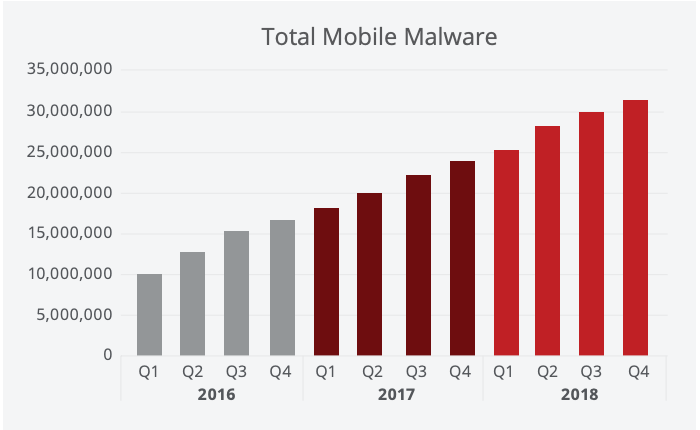
\includegraphics[scale=0.9]{./Figure/androidgraph.png}
    \caption{Total mobile malware \cite{mcafee}}
    \label{fig:androidgraph}
  \end{figure}

In order to mitigate the spread of malware, Google introduced a detection mechanism to its app market in Feb 2012 called Bouncer. Bouncer tests submitted applications in a sandbox for five minutes in order to detect any harmful behaviours; however, it has been shown that bouncer can be evaded by means of some simple detection avoidance methods. Alongside Bouncer, Google introduced Google Play protect in the Google 2017 event \cite{googleplay}. Google Play Protect is an always-on service that scans the applications automatically even after installation to ensure that the installed applications remains harmless 24/7. It has been reported that over 50 billion apps are scanned and verified every day regardless of where they were download from. However, according to McAfee, Google Play Protect also failed when tested against malware discovered in the previous 90 days in 2017 \cite{mcafee2018}. Furthermore, most third-party stores do not have the capability to scan and detect submitted harmful applications. Clearly, there is still a need for additional research into efficient methods to detect zero-day Android malware in the wild in order to overcome the aforementioned challenges.

Cyber attacks manage to produce unprecedented levels of disruption, where attackers usually leverage diverse tools and tactics, such as zero-day vulnerabilities and malware. This situation makes malware detection techniques worth studying and improving, in order to prevent and/or mitigate the effects of cyber attacks. Machine learning techniques can help to satisfy this demand,building classifiers that discern whether a precise Android application is malware or benignware. Algorithms such as Decision Trees, Support-Vector Machines and NaiveBayes, to name a few, are able to build such classifiers. Going further, ensemble methods for machine learning aim at effectively integrating many kinds of classification methods and learners to benefit from each ones advantages and overcome their individual drawbacks, hence improving the overall performance of the classification.

Various approaches have been proposed in previous works with the intention of detecting Android malware. These approaches are categorized into static analysis, dynamic analysis or hybrid analysis (where static and dynamic are used together). The methods based on static analysis reverse engineers the application for malicious code analysis. Arp et al. (2014) \cite{drebin}, M. Yusof et al \cite{apicallpaper}. Fan et al. (2017)\cite{dapasa}, are few examples of detection methods using static analysis. Static analysis of Android malware can rely on Java bytecode extracted by disassembling an application. The manifest file is also a source of information for static analysis. By contrast, dynamic analysis executes the application in a controlled environment such as an emulator, or a real device with the purpose of tracing its behavior. Several dynamic approaches, one of them is Alzaylaee, M.K., Yerima, S. Y., and Sezer S. (2016) DroidBox \cite{andropytool}. However, the efficiency of these approaches rely on the ability to detect the malicious behavior during the runtime while providing the perfect environment to kick-start the malicious code.
And many approaches do not have an end-to-end system to detect malware. They have some separated steps to predict and are not easy to use for users.

In this paper, we will focus on Static analysis methods to detect malware in \ac{apk} using features extracted from these \ac{apk} files with reverse engineering methods. We used a tool named AndroPytool\cite{andropytool} to extract 7 different Static features described at table\ref{table:1}. 


\begin{table}[htbp]
  \centering
  \caption{Static features used in our proposed system}
  \label{table:1}
  \begin{tabular}{|c||l l|}
  \hline
  & \textbf{Feature name} & \textbf{Description}\\
  \hline
  \multirow{7}{4em}{Static Feature}
   & API calls &  Count of system calls performed by an APK \\ 
   & Opcodes & Count of opcodes performed by an APK \\ 
   & Permissions & Which permissions uses the APK \\ 
   & Intent receivers & Set of an APK’s receivers \\ 
   & Intent services & Services used by an application \\
   & Intent activities & Activities declared by an APK \\ 
   & System commands & Set of system commands ran by the app \\ \hline
  
  \end{tabular}
  \end{table}

Using these features, we trained several machine learning models to predict if the application is a malware or not. Then we use these models predictions to train other new models to predict the malware application. This technique is called Stacking. It is a way to ensemble multiple classifications or regression models. This method is often used by data scientists in Kaggle \cite{kaggle} competitions to improve the final prediction and is one of the state-of-art techniques in table data competitions.
Furthermore, we propose an end-to-end system that uses for input an android \ac{apk} and output the result of detection, benign application or malware application. 


\chapter{Background}

\section{Overview of Android OS}

The Android architecture
is structured in a series of layers (see \ref{fig:androidsystem}) offering different components and functionalities at different levels of abstraction, from hardware to system applications.
The bottom layer is composed by the Linux Kernel. This is the core system of Android, on top
of which all the components and layers are deployed. It also manages some of the most important security related policies. The next layer, in ascending order, is the \ac{hal}, in charge of allowing access to the hardware from components in upper layers.
It contains independent modules for each hardware component.

\begin{figure}[htbp]
  \centering
  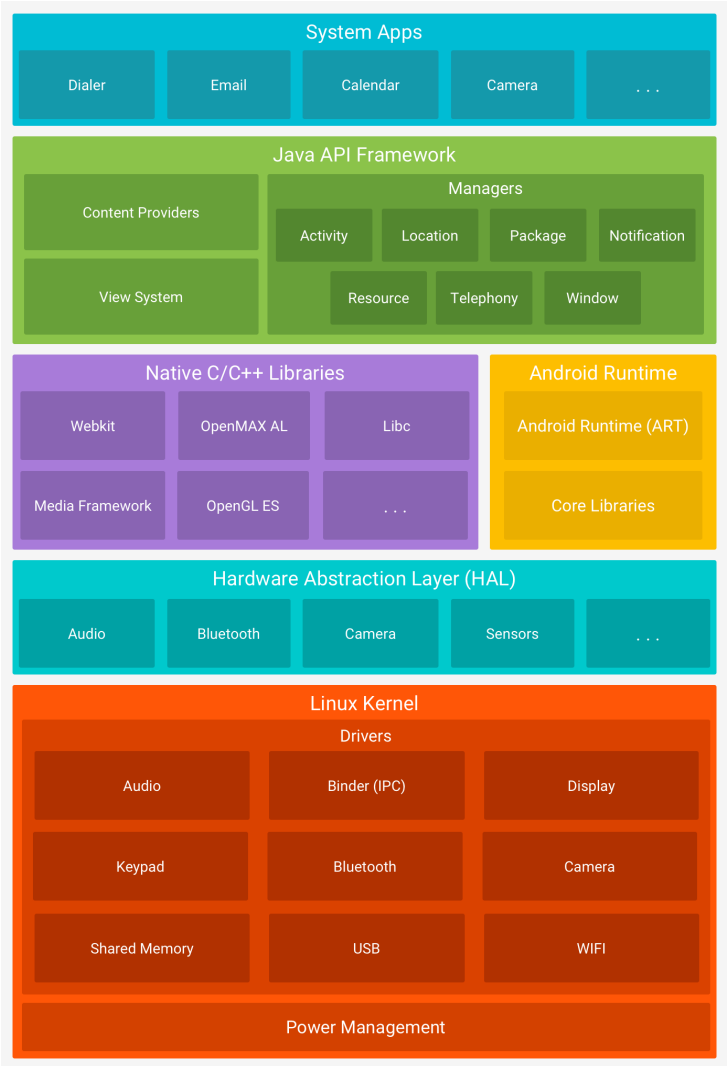
\includegraphics[scale=0.65]{./Figure/androidsystem.png}
  \caption{Android operating system architecture}
  \label{fig:androidsystem}
\end{figure}

Two layers are placed above. The first one, the Native C/C++ Libraries, used by developers who build their applications in any of these programming languages or also employed by
the Java \ac{api}. The second one is the \ac{art}, which has replaced Dalvik.
This environment allows running multiple virtual machines where applications developed in Java
execute in isolation.

On top of the two previously described parallel layers, it is possible to find the Java \ac{api}
framework. Through this \ac{api}, it is possible to access all functionalities offered by the Android
Operating system. The main objective of this layer is to facilitate the process of developing new
applications or reusing code in a rich environment designed to help the developer. Finally, the
top layer contains a set of system applications. They provide basic functionalities to the user,
such as internet browser, phone, email or calendar, but they can be replaced by other applications
installed by the user.

In Android, applications are distributed in files with extension .apk, which stands for \ac{apk}. These compressed files in zip format contain the necessary code, data, and
resources required to execute the application. 

\section{APK file structure}

\begin{figure}[htbp]
  \centering
  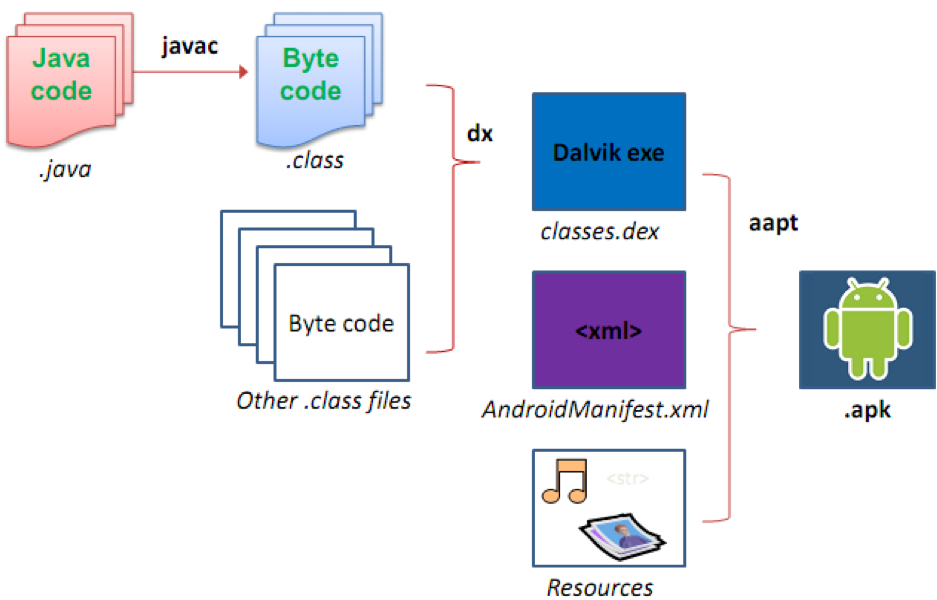
\includegraphics[scale=0.6]{./Figure/apkfile.png}
  \caption{Overview of the different files and folders obtained after unzipping an \ac{apk}}
  \label{fig:apk}
\end{figure}

Figure\ref{fig:apk} presents an overview of the different files and folders obtained after unzipping an \ac{apk}. However, since some of these files contain encrypted information, it is required to use specific tools such as AndroGuard \cite{androguard} or Apktool\cite{apktool} to extract the human readable
version of each file. The files contained in the different folders provide varied information which
can be used to categorize the behavior of the sample. For instance, /META-INF/ includes certificates, developer information or information to run the jar file. /assets/, resources.arsc and
/res/ are related to different mechanisms to import resources. The /lib/ folder stores compiled
libraries. Finally, two files provide the most relevant features when facing a malware analysis
task and which are shown in Figure\ref{fig:androidsystem}. classes.dex defines the code of the application in the
form of Dalvik bytecode. From here, a list of API calls, system commands or receivers defined
can be retrieved. The second important file is the AndroidManifest.xml, which declares a list of
permissions, the package name or a relation of intent filters.

\section{Android Malware}

Android malware applications primarily consist of
Trojans. A typical Android Trojans might trick the
user by using icons or user interfaces that mimic a
benign application. Android Trojans often display a
service level agreement during installation which
obtains permissions to access a user’s personal
information, such as the phone number. The Trojan
can then, for example, send SMS to premium rate
numbers in the background.
Android Trojans are also often used as spyware.
Such malicious applications can gain access to a
user’s private information and send it to a private
server. The main purpose of such spyware is to steal
information such as phone location, bank or credit
card details, passwords, text messages, contacts,
online browsing activity, and so on. A more
sophisticated implementation might also include
botnet capabilities.


\section{Analysis techniques for applications}
\subsection{Static Analysis}
In the static analysis, the analysis of the applications is done and the features are extracted without executing the application on an emulator or device. In comparison to other analysis techniques for android malware detection, static analysis consumes fewer resources and time as it does not involves execution of the application. The major disadvantage of this analysis is code obfuscation because of which detecting the malicious behavior of the application becomes difficult as pattern matching is not possible. This analysis can detect runtime errors, logical inconsistencies, and possible security violations.

Also static analysis includes the use of
reverse engineering techniques in order to access the set of instructions that define the application
operation. Furthermore, and focused on the Android platform, a large variety of characteristics
can be revealed using this kind of analysis. Information gathered from the Android Manifest or
from the resources are included into this category.

\subsection{Dynamic Analysis}

Dynamic analysis is the testing and evaluation of a program by executing data in real-time. The objective is to find errors in a
program while it is running, rather than by repeatedly examining the code offline. It is a detection technique which aims at
evaluating malware by executing the application and the main advantage of this technique is that determines the application
behavior during runtime and loads target data. The resource consumption in this analysis technique is more as compared to static
analysis. Dynamic behavioral detection method constructs operation environment by using a sandbox, virtual machine, and other
forms, and simulates the execution of the application to acquire the application’s behavior model.

\subsection{Hybrid Analysis}

Hybrid Analysis is a combination of static and dynamic analysis. It is a technology or method that can integrate run-time data
extracted from dynamic analysis into a static analysis algorithm to detect behavior or malicious functionality in the applications.
The hybrid analysis method involves combining static features obtained while analyzing the application and dynamic features and
information extracted while the application is executed. Though it could increase the accuracy of the detection rate, it makes the
system cumbersome and the analysis process is time consuming. 

\section{State-of-the-art machine learning algorithms for Android malware detection}

This section summarizes the most used machine learning classification algorithms in the literature
related to Android malware detection and family classification.

\subsection{Decision Trees}

Decision trees are one of the former machine learning methods for regression and classification.
They provide a useful mechanism based on a set of splitting rules. These models make
a prediction based on the most common class in the region of the example. Typically, decision
trees are generated through consecutive binary splitting while an error function is minimized. One
of the strengths of these models lies in that they allow an easy interpretation and visualization.
In contrast, they have several drawbacks, such as classification problems when presenting data
with small changes. An example of decision tree algorithm is ID3, which makes divisions
trying to maximize the information gain.

\subsection{Random Forest}

Decision trees are one of the simplest learning
techniques. However, a decision tree tends to overfit
the training data, since it is a literal interpretation of
the data, and provides no generalization of the training set. To partially alleviate this problem,
multiple decision trees can be used, where each is
trained on a subset of the training data. A random
forest takes this idea one step further by also training
on subsets of the classifiers \cite{breiman}.
Although much of the inherent simplicity of decision
trees is lost in this process, random forests have
proved to be a very strong machine learning
technique over a wide variety of applications. 

\subsection{K-nearest neighbors}

The K-nearest neighbors is a non-parametric classifier, meaning that this model grows in parallel
to the size of the training data \cite{rob14}. Basically, it uses a distance metric to provide a prediction
based on the majority class among the K nearest point to the example. While these models have
proved to be powerful in varied problems, they are not indicated for high-dimensional spaces.

\subsection{Support Vector Machine}

This is a powerful algorithm used for both classification and regression problems. It is based on
representing each example in a n-dimensional space, where a hyperplane is created pursuing the
best separation between classes \cite{svm}. For building this hyperplane, a portion of the training
data called support vectors is employed. These models have been widely used in the literature
for building malware detection tools.

\subsection{Logistic Regression}

Logistic regression is the appropriate regression analysis to conduct when the dependent variable is dichotomous (binary). \cite{logic} Like all regression analyses, the logistic regression is a predictive analysis.  Logistic regression is used to describe data and to explain the relationship between one dependent binary variable and one or more nominal, ordinal,interval or ratio-level independent variables.

\subsection{Gradient boosting}
Gradient boosting is a machine learning technique for regression and classification problems, which produces a prediction model in the form of an ensemble of weak prediction models, typically decision trees. It builds the model in a stage-wise fashion like other boosting methods do, and it generalizes them by allowing optimization of an arbitrary differentiable loss function.

Nowadays we have some state-of-the-art algorithms implementing Gradient boosting.
Below, we introduce the top 3 of the most used algorithm implementing Gradient boosting.

\subsubsection{XGBoost}

XGBoost is an algorithm that has recently been dominating applied machine learning and Kaggle competitions for structured or tabular data.

XGBoost is an implementation of gradient boosted decision trees designed for speed and performance created by Tianqi Chen, now with contributions from many developers. \cite{xgboost}

\subsubsection{LightGBM}

LightGBM is a gradient boosting framework that uses tree based learning algorithms. It is designed to be distributed and efficient with the following advantages: Faster training speed and higher efficiency,
Lower memory usage,
Better accuracy,
Support of parallel and GPU learning,
Capable of handling large-scale data. \cite{lgbm}

\subsubsection{Catboost}

CatBoost is an algorithm for gradient boosting on decision trees. It is developed by Yandex researchers and engineers, and is used for search, recommendation systems, personal assistant, self-driving cars, weather prediction and many other tasks at Yandex and in other companies, including CERN, Cloudflare, Careem taxi. It is in open-source and can be used by anyone. \cite{cat}

\subsection{Artificial Neural Networks}

Artificial neural networks are algorithms that can be used to perform nonlinear statistical modeling and provide a new alternative to logistic regression, the most commonly used method for developing predictive models for dichotomous outcomes in medicine. Neural networks offer a number of advantages, including requiring less formal statistical training, ability to implicitly detect complex nonlinear relationships between dependent and independent variables, ability to detect all possible interactions between predictor variables, and the availability of multiple training algorithms. \cite{neuralnets}
\chapter{Methodology}

In this chapter, we describe the methodology of our proposed Android malware detection system based on static features and how we implemented our models using our proposed Stacking method.

\section{Dataset} \label{dataset}

To begin with this Chapter we will introduce the dataset used in this paper. We used a dataset called Androzoo.
AndroZoo is a growing collection of Android Applications collected from several sources, including the official Google Play app market.
It currently contains 10,299,119 different APKs, each of which has been (or will soon be) analyzed by tens of different AntiVirus products to know which applications are detected as Malware\cite{androzoo}.

Due to keeping a balanced dataset containing both malware and benignware samples,
We collected 10,000 malware \ac{apk}s and 10,000 benignware samples randomly from the above dataset Androzoo. Also, we have done a filtering process in which we remove repeated applications and those that are considered as invalid (they cannot be actually installed and executed). After removing these applications we download again the remaining number to complete 10,000 of \ac{apk}s and done the filtering process again. We repeated these steps until to gather a clean dataset consisted of 10,000 \ac{apk}s of malware applications and 10,000 \ac{apk}s of benignware applications with a total of 20,000 \ac{apk}s.

\section{Static Features extraction} \label{extractedvector}

Static features focus on a large part of the state-of-the-art literature related to Android malware
detection. The easy and quick extraction of this kind of feature makes them suitable to be used to build malware detection tools.

One of our system goals is to do a prediction process while the user only needs to input the \ac{apk} file to receive the output (malware or not). In other words, it is called an end-to-end system. One essential process to achieve this goal is, we have to automatically the feature extraction process and convert it to vectors that the machine learning models could use for inputs to predict something.
So in this study, we use an opensource tool called AndroPytool \cite{andropytool}.

AndroPyTool can extract static and dynamic features, this section focuses on the
former ones. By using Android malware analysis tools such as AndroGuard or by analyzing the source code of each sample, AndroPyTool extracts a representative set of characteristics based on state-of-the-art Android malware detection approaches. These features include API calls, main activity name, opcodes, package name, permissions, intent receivers, intents services, intent activities, strings found, system commands or information flows extracted with FlowDroid.

Once extracted the desired set of characteristics, such as permissions requested, API calls
invoked or information flows, all this information is processed to build a representative feature
vector for each application. This process is shown in Fig. \ref{fig:featurevector} On the one hand, $M$ measurable
characteristics $$ C_{M}=\left\{c_{1}, c_{2}, \ldots, c_{M}\right\} $$ are assigned a value counting the number of occurrences of
that feature within the application. On the other hand, $K$ binary features $$
D_{K}=\left\{d_{1}, d_{2}, \ldots, d_{K}\right\}
$$
point the use or the existence of a particular attribute. The bundling of both features composes
the static description of the application behavior, in other words, our input dataset $\mathcal{D}$.
$$
\mathcal{D}=\left\{\mathbf{x}_{i}, y_{i}\right\} \text{where }
\mathbf{x}_{i}=\left\{c_{1,}^{i} c_{2}^{i}, \ldots, c_{M}^{i}, d_{l,}^{i}, d_{2}^{i}, \ldots, d_{K}^{i}\right\}
$$

\begin{figure}[htbp]
    \centering
    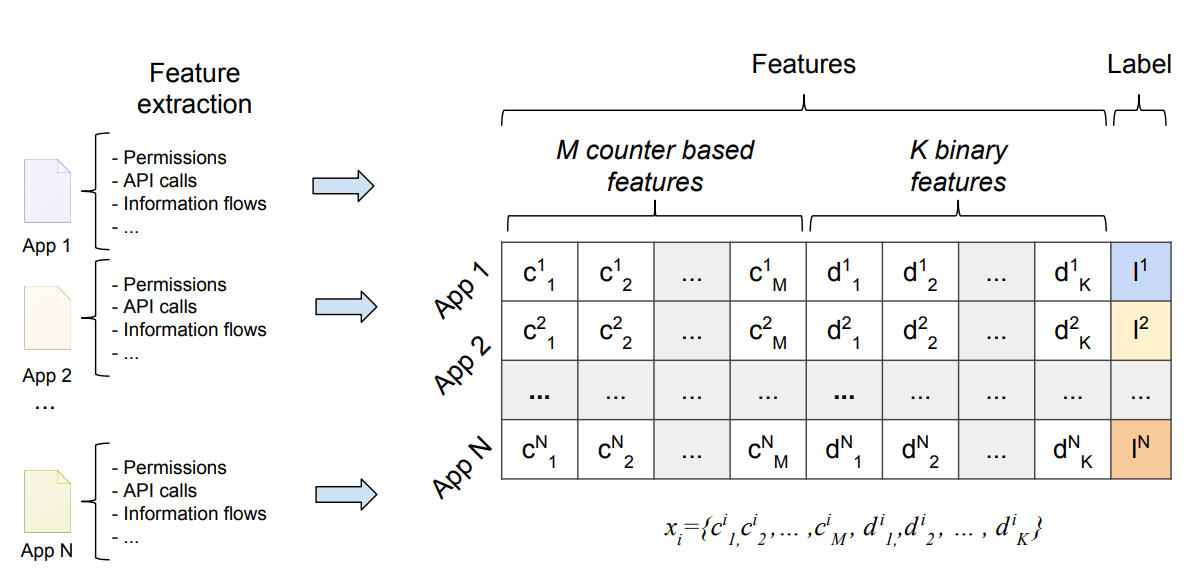
\includegraphics[scale=0.68]{./Figure/featurevector.png}
    \caption{Extraction and representation of static information into representative feature vectors. \cite{andropytool}}
    \label{fig:featurevector}
\end{figure}


\section{Stacking}
Stacking is an ensemble learning technique that combines multiple classifications or regression models via a meta-classifier or a meta-regressor \cite{stackingref}. The base level models are trained based on a complete training set, then the meta-model is trained on the outputs of the base level model like features as we can see in Figure \ref{fig:stacking}.

\begin{figure}[htbp]
    \centering
    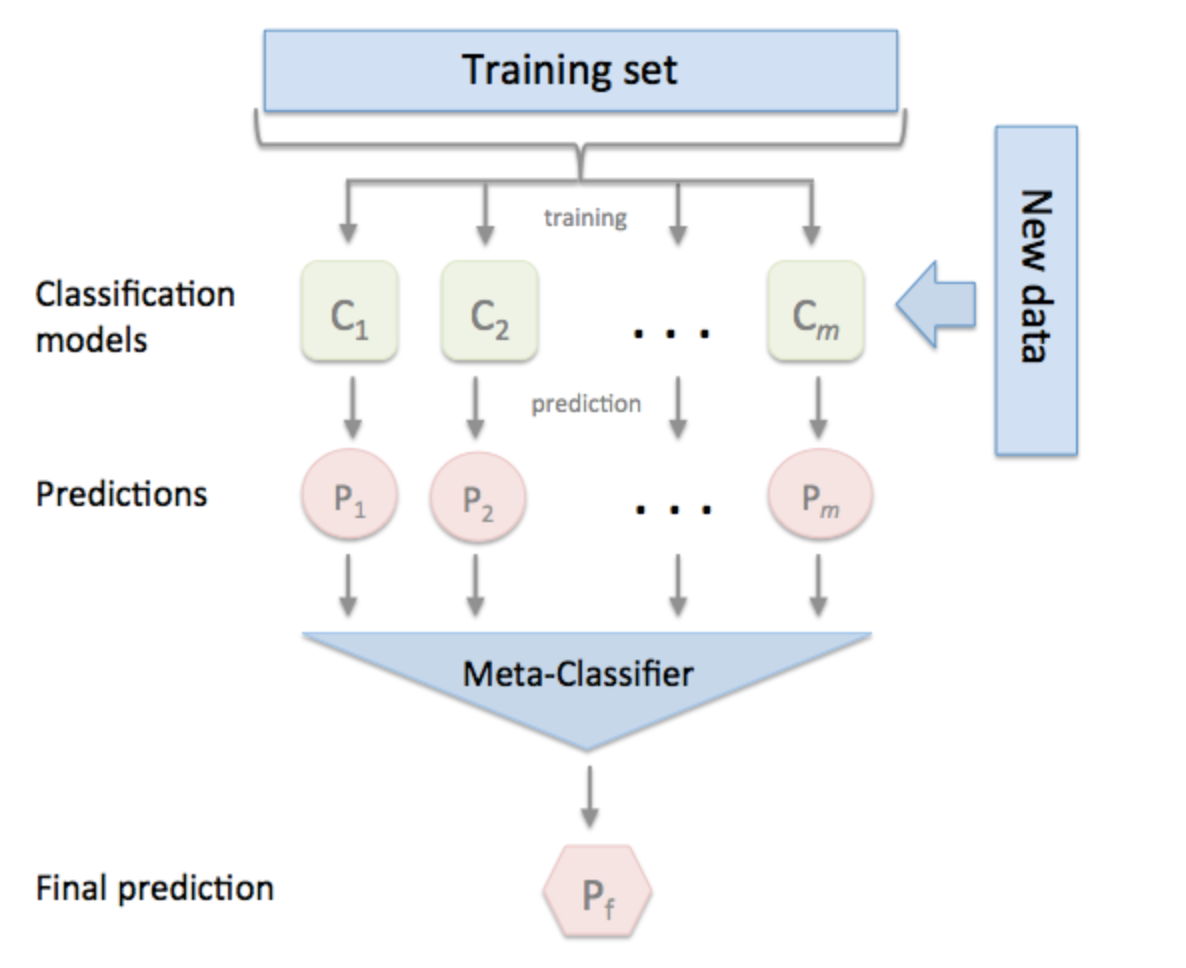
\includegraphics[width=\textwidth]{./Figure/stacking.png}
    \caption{Stacking pipeline figure.}
    \label{fig:stacking}
\end{figure}


The base level often consists of different learning algorithms and therefore stacking ensembles are often heterogeneous. But we must note that this type of Stacking is prone to overfitting due to information leakage. We should not derive the predictions for the 2nd-level classifier from the same dataset that was used for training the level-1 classifiers. The algorithm \ref{alg:algo1} summarizes stacking.

\begin{algorithm}[htbp]
    \centering
    \caption{Stacking}
    \label{alg:algo1}
    \begin{algorithmic}[1]  
    \renewcommand{\algorithmicrequire}{\textbf{Input:}}
    \renewcommand{\algorithmicensure}{\textbf{Output:}}
    \Require Training data $\mathcal{D}=\left\{\mathbf{x}_{i}, y_{i}\right\}_{i=1}^{m}\left(\mathbf{x}_{i} \in \mathbb{R}^{n}, y_{i} \in \mathcal{Y}\right)$
    \Ensure An ensemble classifier $H$
    \State Step 1: Learn first-level classifiers
    \For{$t\gets$ 1 to $T$}
        \Statex Learn a base classifier $h_{t}$ based on $\mathcal{D}$
    \EndFor
    \State Step 2: Construct new data sets from $\mathcal{D}$
    \For{$i = 1$ to $m$}
    \State $\text{Construct a new data set }\mathcal{D}_{h}=\left\{\mathbf{x}_{i}^{\prime}, y_{i}\right\}, \text { where } \mathbf{x}_{i}^{\prime}=\left\{h_{1}\left(\mathbf{x}_{i}\right), \ldots, h_{T}\left(\mathbf{x}_{i}\right)\right\}$
    \EndFor
    \State Step 3: learn a meta-classifier
    \State Learn a new classifier $h^{\prime}$ based on the newly constucted data set $\mathcal{D}_h$
    \State \textbf{return} $H(\mathbf{x})=h^{\prime}\left(\mathcal{D}_h\right)$
    \end{algorithmic}
\end{algorithm}

Besides, Stacking is a commonly used technique for winning the Kaggle data science competition. For example, the first place for the Otto Group Product Classification challenge was won by a stacking ensemble of over 30 models whose output was used as features for three meta-classifiers: XGBoost, Neural Network, and Adaboost.

\section{Proposed model pipeline} \label{model}

In this section, we will introduce the main topic of our system, the Stacking model pipeline as we can see in Figure\ref{fig:modelpipeline}. Our proposed model consists of 3 stages with different models to predict one final output.

\begin{figure}[htbp]
    \centering
    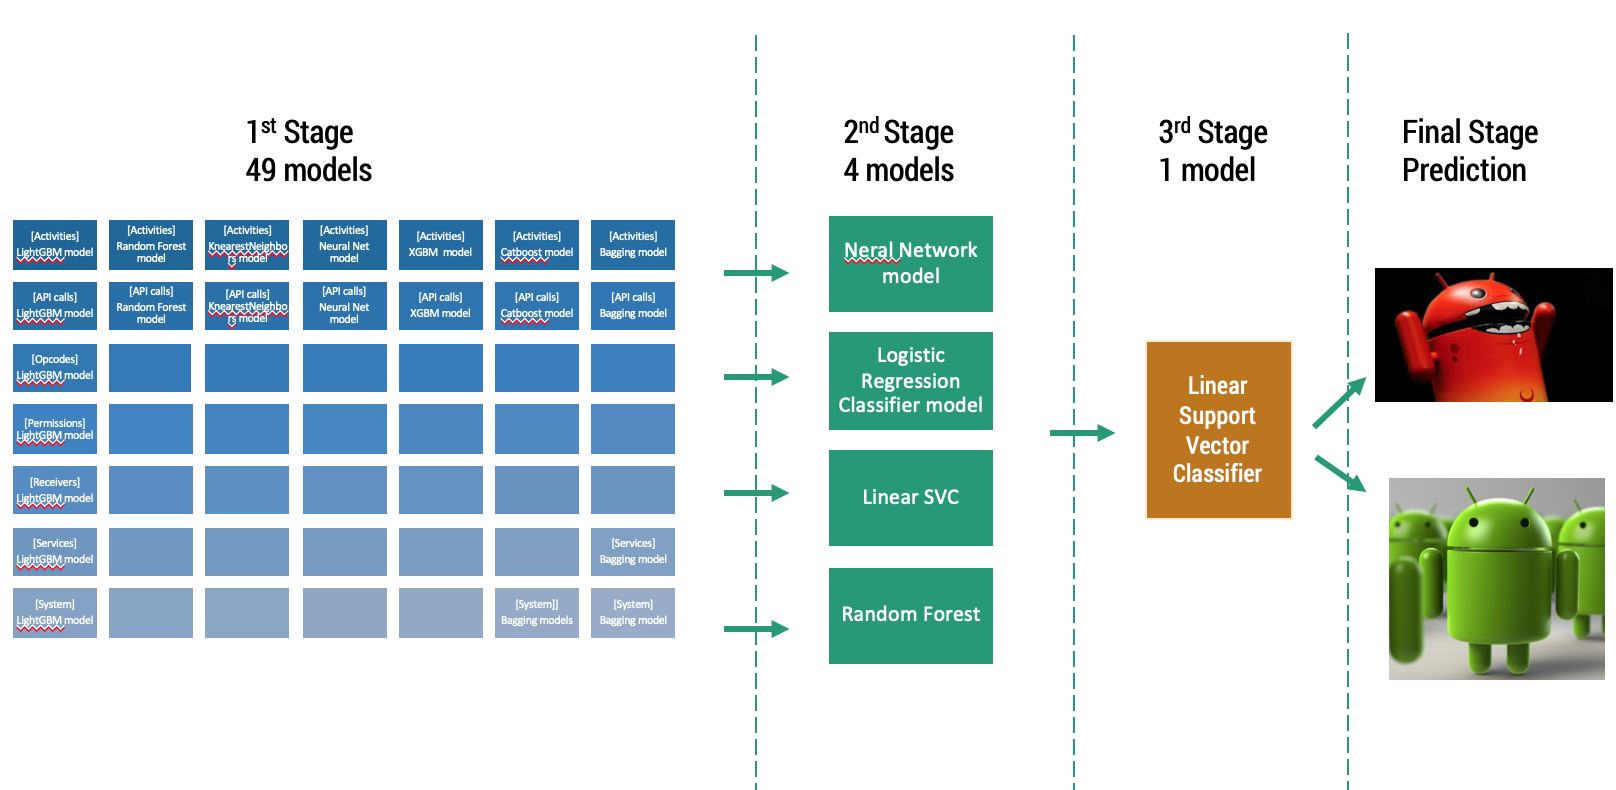
\includegraphics[width=\textwidth]{./Figure/modelpipeline.png}
    \caption{Proposed Stacking model pipeline figure.}
    \label{fig:modelpipeline}
\end{figure}

\subsection{1st Stage}
For this first stage, we proposed to train 7 different algorithms (Bagging, XGBoost, K-neighbors, LogisiticRegression, RandomForest NeuralNetworks) to each 7 different static feature (Activities, API calls, Opcodes, Permissions, Receivers, Services, System commands) to create our models of a total of 49 models. 

Following the Algorithm \ref{alg:algo1}, we trained the base 49 classifiers $h_{t=49}$ on our training dataset as mentioned in section \ref{dataset}. Where our input training data is $\mathbf{x}_{i}$ and label data is $y_{i}$
 $$\left\{\mathbf{x}_{i}, y_{i}\right\}_{i=1}^{m=7}\left(\mathbf{x}_{i} \in \mathbb{R}^{n}, y_{i} \in \mathcal{Y}\right)$$


Due to every model has one output for one \ac{apk} input, we gain one output vector from $\mathcal{D}$ as we can see at below $$\mathcal{D}_h = \left\{\mathbf{x}_{i}^{\prime}, y_{i}\right\}, \text { where } \mathbf{x}_{i}^{\prime}=\left\{h_{1}\left(\mathbf{x}_{i}\right), \ldots, h_{T=49}\left(\mathbf{x}_{i}\right)\right\}$$

\subsection{2nd Stage}
In this stage, we proposed to train 4 different algorithms (Neural Network, Logistic Regression classifier, Linear SVC, RandomForest) with the output vector from the 1st stage as input data.
Following the Algorithm \ref{alg:algo1}, we train our 2nd stage meta-classifiers $H_{k}$($k=4$) based on the newly constructed data set at 1st stage $\mathcal{D}_h$. Then we obtained the below models $H_{k}$
$$H_{k}(\mathbf{x})=h^{\prime}\left(\mathcal{D}_h\right)$$



\subsection{3rd Stage}
In this stage, we repeated the 2nd stage process using $H_{k}\left(\mathbf{x}\right)$ as input to train our final meta-classifier (Linear SVC).

We trained our final meta-classifier $L$ based on the newly constructed dataset at 2nd stage $\mathcal{D}_l = \left\{\mathbf{h}_{i}^{\prime}, y_{i}\right\}$. Then we obtain the below trained final meta-classifier $L\left(\mathbf{x}\right)$
$$L(\mathbf{x})=l^{\prime}\left(H_{1}(\mathbf{x}), H_{2}(\mathbf{x}), \ldots, H_{k}(\mathbf{x})\right)$$



\section{Proposed Malware detection System}
In this section, we introduce our proposed malware detection system implementing our proposed Stacking model in section \ref{model}. We can see the overview of our proposed system pipeline in Figure \ref{fig:systempip}.

\begin{figure}[htbp]
    \centering
    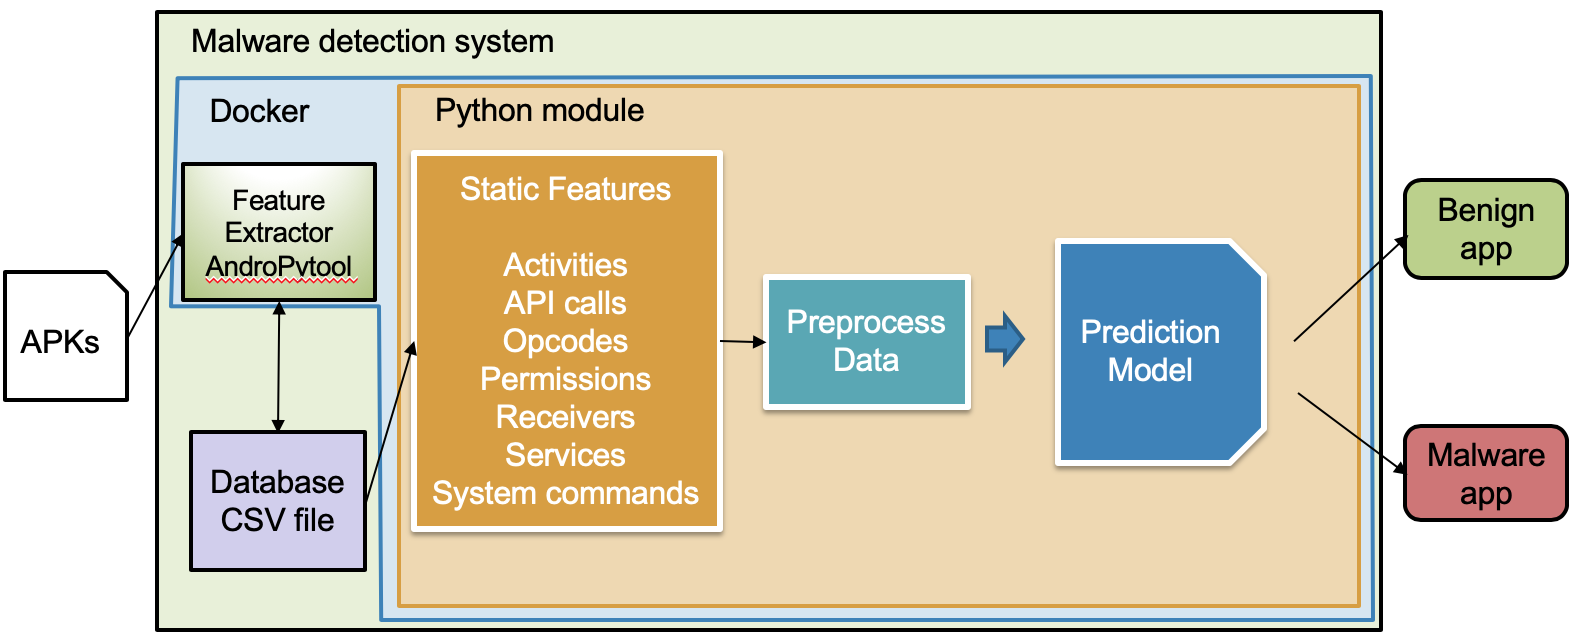
\includegraphics[width=\textwidth]{./Figure/systempip.png}
    \caption{Proposed malware detection system pipeline figure.}
    \label{fig:systempip}
\end{figure}

\subsection{AndroPytool module}

We build almost all of this system in a Linux Docker container. The main merit of building a system with Docker is that it makes easy for the users to deploy this system in other environments not needing to care about dependent packages. 

First, we implemented the AndroPyTool\cite{andropytool} module. Here we input the APK file to extract the static features to our database as \ac{csv} file, as we can see in section \ref{extractedvector}.  

\subsection{Preprocessing data}

Next, we load the extracted features from our database to our python module.
In this module, we preprocess our data (static features in vectors) before to input it into our classifier model. We applied two steps to preprocess our data.

\subsubsection{Standard scaling}
In the first step, we applied the Standard scaling to all of our counter-based features. Below is the formula applied for Standard scaling.

$$x^{\prime}=\frac{x-\bar{x}}{\sigma}$$

Where $x$ is the original feature vector, $\bar{x}=average(x)$ is the mean of that feature vector, and $\sigma$ is its standard deviation.

\subsubsection{One-hot encoding}
For the second step, we applied One hot encoding method to our categories features or binary features. 
One hot encoding is a process by which categorical variables are converted into a form that could be provided to ML algorithms to do a better job in prediction.
The figure \ref{fig:onehotexample} explain the One hot encoding process. In this example, we applied One hot encoding to the CompanyName collum. After converting the CompanyName to CategoricalValue it is converted to binary values.

\begin{figure}[htbp]
    \centering
    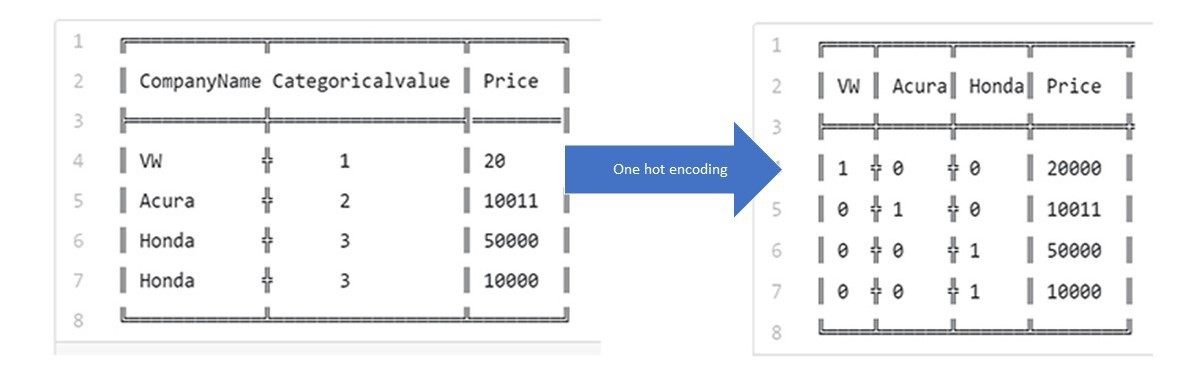
\includegraphics[width=\textwidth]{./Figure/onehotexample.png}
    \caption{One hot encoding explained in an image.}
    \label{fig:onehotexample}
\end{figure}

\subsection{Prediction of malware}

After preprocessing our data to the best format for all of our classifiers, finally, we do the malware prediction step.
We input the preprocessed data to the 49 models as mentioned in section \ref{model}.
After the 3 steps of prediction, the final classifier outputs the final prediction (0 for Benign app, 1 for Malware app).


\chapter{Experiments and Results}
The main aim of this section is to assess the use of static features when involved in the characterisation of Android malware and benignware samples used to train detection tools. Thus, through
the use of several machine learning classifiers, it is studied if this combination with stacking methods is feasible and, if
so, to assess its performance when applied to build a machine learning aided Android malware
detection tools.

\section{1st Stage training experiments} \label{1ststagetrain}

For the 1st stage training step of our model, the selected ensemble classifiers were run with the Scikit-learn library for Python\cite{scikitlearn}.
They include AdaBoost, XGBoost, Catboost, Bagging Classifier, K-nearest neighbors, Neural network, Random Forest. 
All these ensemble classifiers were tested with the previously mentioned dataset through a 10-folds cross validation with accuracy scoring method showed below.

$$Accuracy = (TP+TN)/(TP+TN+FP+FN)$$
$$where: TP = \text{True positive}; FP = \text{False positive};$$$$TN = \text{True negative}; FN = \text{False negative}$$

For a better evaluation of the capacity of these algorithms to extract
and generalise conclusions, several experiments were conducted in order to judge the individual performance of the all models.
The results are shown in Table \ref{table:1ststage} and Figure \ref{fig:1ststage}

\begin{table}[htbp]
    \centering
    \caption{Experiments results on 1st training stage}
    \label{table:1ststage}
    \begin{adjustbox}{width=\textwidth}
        
    \begin{tabular}{|cccccccc|}
        \hline
        
        \textbf{Model} & \textbf{Activities CV} & \textbf{API calls CV} & \textbf{Opcodes CV} & \textbf{Permissions CV} & \textbf{Receivers CV} & \textbf{Services CV} & \textbf{System CV} \\ \hline
        LightGBM & 0.5094 & 0.8783 & 0.8519 & 0.7979 & 0.8486 & 0.5094 & 0.7866 \\ \hline
        Bagging & 0.5108 & \textbf{0.8817} & 0.8544 & 0.8094 & 0.8577 & 0.5099 & 0.7986 \\ \hline
        CatBoost & 0.5103 & 0.8762 & 0.8499 & 0.8048 & 0.8525 & 0.5031 & 0.7912 \\ \hline
        Neural Network & 0.5124 & 0.8518 & 0.8189 & 0.7841 & 0.8429 & 0.5092 & 0.7692 \\ \hline
        XGBoost & 0.5099 & 0.8740 & 0.8469 & 0.8008 & 0.8388 & 0.5094 & 0.7809 \\ \hline
        Random Forest & 0.5098 & 0.8238 & 0.8348 & 0.6143 & 0.7946 & 0.5064 & 0.7526 \\ \hline
        K-Neighbors & 0.5050 & 0.8466 & 0.8279 & 0.7817 & 0.8440 & 0.5116 & 0.7743 \\ \hline
        
        \end{tabular}

    \end{adjustbox}
    \end{table}

    \begin{figure}[htbp]
        \centering
        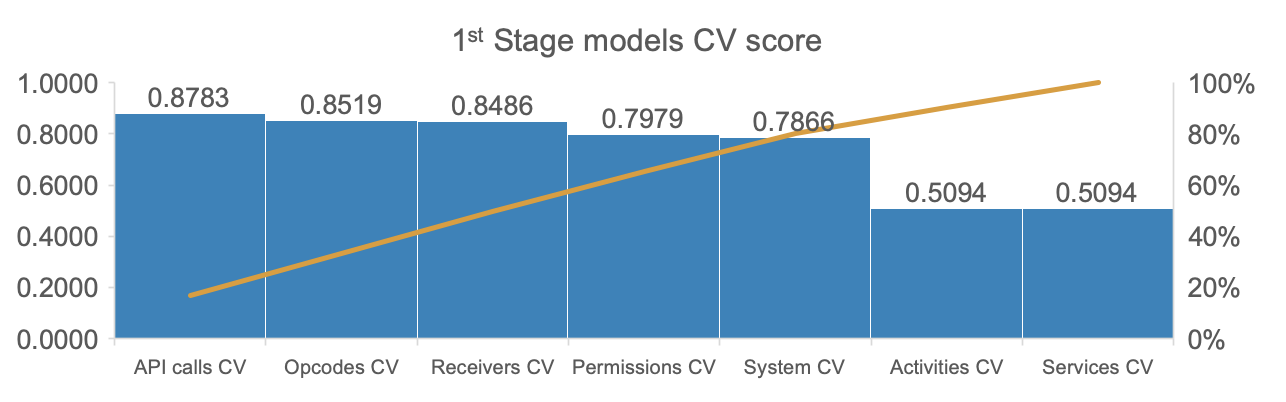
\includegraphics[width=\textwidth]{./Figure/1ststage.png}
        \caption{1st Stage models CV accuracy score average}
        \label{fig:1ststage}
      \end{figure}

 In particular, API
calls compose the most appropriate representation to build a machine learning classification
tool, exhibiting a 88.17\verb+%+ accuracy with a Bagging classifier. In general,
this algorithm obtains the best results overall.
% It is remarkable the fact that a combination of API calls with other also competitive features,
% such as opcodes or receivers, which have proved to be powerful at building detection mechanisms, does not lead to better values.

It is remarkable the fact that not only API calls has good results but also Opcodes and Receivers have proved to be powerful at building detection mechanisms as we can see in Figure \ref{fig:1ststage}. In contrast, we found that Activities and Services are to be less useful at building malware detection mechanisms.

\section{2nd Stage training experiments}

In the 2nd stage for training we used the predictions results of the 1st stage as input to training our 4 selected classifiers. Due to we have only 49 inputs to each model, we selected 4 algorithms that are good to handle with small datasets. It are Neural Network, Logistic Regression Classifier, Linear SVC, Random Forest.
All these classifiers were tested with the previously mentioned dataset through a 10-folds cross validation with accuracy scoring method as section \ref{1ststagetrain}.
The results are shown in the Table \ref{table:2ndstage} and Figure \ref{fig:2ndstage}.


\begin{table}[htbp]
    \centering
    \caption{Experiments results on 2nd training stage}
    \label{table:2ndstage}
        
        \begin{tabular}{|cc|}
            \hline
            
            \textbf{Model} & \textbf{CV score} \\ \hline
            \textbf{LinearSVC} & \textbf{0.9356} \\ \hline
            \textbf{RandomForestClassifier} & \textbf{0.9339} \\ \hline
            \textbf{Neural Network} & \textbf{0.9334} \\ \hline
            \textbf{LogisticRegression} & \textbf{0.9312} \\ \hline
            1st Stage best model & 0.8817 \\ \hline
            
            \end{tabular}
    \end{table}

    \begin{figure}[htbp]
        \centering
        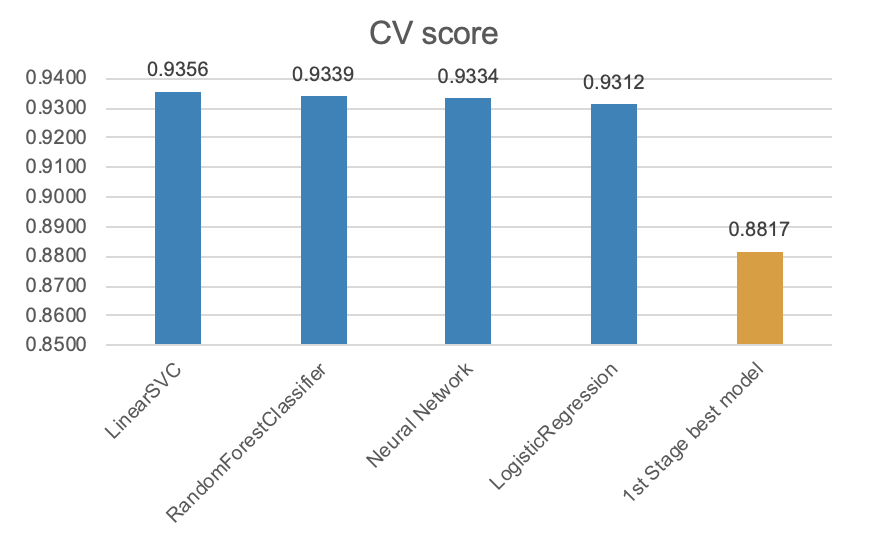
\includegraphics[scale=0.8]{./Figure/2ndstage.png}
        \caption{2nd Stage models CV accuracy score}
        \label{fig:2ndstage}
      \end{figure}

From these results of 2nd stage we could see that our all models score are better than the best score from 1st stage. Moreover, comparing to the best model at this stage we have a difference of about 5.39\verb+%+ from the 1st stage best model. This fact could prove that our Stacking method is useful and very powerful method to improve the performance of malware detection systems or models.
\chapter{Conclusion}


% % %
% End of Body
% % %

% % Bibliography style
\singlespacing
\bibliographystyle{IEEEtran}
\bibliography{ref}
% % If you add references to a table of contents, uncomment the following line
% \addcontentsline{toc}{chapter}{References}

% % You can make appendixes, if any.
% \appendix
% \include{./Chapter/hogehoge.tex}

\end{document}
